
\documentclass[12pt,a4paper]{article}

% ---------------------------------------------------------------------------
% Packages
% ---------------------------------------------------------------------------
\usepackage[top=2.5cm, bottom=2.5cm, left=3cm, right=3cm]{geometry}
\usepackage{setspace}
\usepackage{booktabs}
\usepackage{tabularx}
\usepackage{threeparttable}
\usepackage{amsmath}
\usepackage{natbib}
\usepackage[hidelinks]{hyperref}
\usepackage{graphicx}
\usepackage{float}
\usepackage{caption}
\usepackage[table]{xcolor}
\usepackage{lscape}
\usepackage{microtype}
\usepackage{siunitx}
\usepackage{footnote}

\onehalfspacing
\bibliographystyle{apalike}

% ---------------------------------------------------------------------------
\begin{document}

\title{CBAM Spillovers and the Industrial Design of Carbon Pricing Instruments}
\author{[Author placeholder]}
\date{\today}
\maketitle

\begin{abstract}
\noindent
Does the EU Carbon Border Adjustment Mechanism shape global carbon pricing adoption and the sectoral design of new instruments? Using a World Bank State \& Trends panel (161 CPIs, 2016--2026), BACI bilateral trade data (196 countries, 2014--2024), and WDI/WGI controls, we find three headline results. First, CBAM-exposed countries advance faster through the carbon pricing pipeline: Cox hazard ratios for the development transition reach 1.20 ($p<0.01$). Second, the 2019 cohort of new instruments shows markedly higher CBAM exposure (mean 2.1\%, ten times the 2016--2018 average) and a 100\% industry coverage rate. Third, panel difference-in-differences coefficients for industry coverage are consistently positive but imprecisely estimated given 49 country clusters. These results are directionally consistent with CBAM driving industry-oriented instrument design, motivating continued panel extension as the mechanism transitions to full implementation.

\medskip
\noindent \textbf{JEL codes:} Q54, Q58, F18, H23
\end{abstract}

\newpage

% ============================================================================
% SECTION 1 — INTRODUCTION
% ============================================================================
\section{Introduction}\label{sec:intro}

The EU Carbon Border Adjustment Mechanism creates a direct financial incentive for non-EU countries to establish domestic carbon pricing. Under Article~9 of Regulation (EU) 2023/956, importers may deduct from their CBAM certificate obligations any carbon price already paid in the country of origin \citep{CBAM2023}. This rebate mechanism means that exporting countries without domestic carbon pricing effectively transfer carbon tax revenues to the EU treasury. Whether this incentive has accelerated both carbon pricing adoption and specifically industry-oriented instrument design is the central empirical question of this paper. The EU accounts for roughly 6\% of global emissions; the CBAM mechanism matters for climate policy only if it catalyses broader policy diffusion beyond Europe's borders.

We find three headline results. First, countries with greater CBAM trade exposure advance faster through the carbon pricing policy pipeline: Cox proportional hazard models yield a hazard ratio of 1.201 ($p<0.01$) for the development transition, meaning a one percentage point increase in CBAM exposure is associated with a 20\% higher hazard of moving into active carbon pricing development (Table~\ref{tab:cox}). Second, the 2019 entrant cohort---twelve new instruments entering the World Bank database in the year the European Commission first announced detailed CBAM plans---shows a mean CBAM exposure of 2.1\%, ten times higher than the 2016--2018 cohorts, with 100\% industry sector coverage from inception (Table~\ref{tab:entrant_desc}). Third, CPI-level panel difference-in-differences estimates for industry coverage are consistently positive (coefficients of +0.97 to +1.11) but imprecisely estimated with 49 country clusters (Table~\ref{tab:panel_did}).

Our work extends the framework of \citet{Bahi2026}, who establish that more CBAM-exposed countries were more likely to adopt some form of national carbon pricing after 2019, using a country-year two-way fixed effects (TWFE) design with a binary adoption outcome. We build on their contribution in two directions. First, we test whether the policy response is visible across the full pipeline from consideration through development to implementation using event-history models, moving beyond the binary adoption indicator. Second, we introduce a sectoral dimension---testing whether new instruments in more-exposed jurisdictions are more likely to cover CBAM-relevant industrial sectors from inception. The binary country-level outcome in \citet{Bahi2026} cannot distinguish between a country that adopts a power-sector-only carbon tax and one that adopts an industry-covering ETS specifically in response to CBAM incentives.

The remainder of this paper is organised as follows. Section~\ref{sec:data} describes the data and measurement. Section~\ref{sec:strategy} presents the empirical strategy. Section~\ref{sec:results} reports results by analytical layer. Section~\ref{sec:robustness} presents robustness checks. Section~\ref{sec:conclusion} concludes.


% ============================================================================
% SECTION 2 — DATA AND MEASUREMENT
% ============================================================================
\section{Data and Measurement}\label{sec:data}

\subsection{Carbon Pricing Instrument Panel}\label{sec:cpi_panel}

Our primary data source is the World Bank \textit{State and Trends of Carbon Pricing} data series \citep{WorldBank2025}. We construct a panel covering 161 carbon pricing instruments (CPIs) across 11 annual editions (S\&T16 through S\&T26, publication years 2016--2026). For each CPI and year we record nine binary sector coverage indicators: power, industry, road transport, aviation, shipping, buildings, waste, agriculture, and forestry. These are parsed from comma-separated sector strings in the source data. We also record time-varying policy status anchored to master-list dates: under consideration start, under development start, and implementation start. These master-list dates differ from first database appearance for some instruments---we document a median gap of 0 years between master-list development start and first sectoral coverage database entry, with Japan's national ETS showing a three-year gap as a concrete example. Annual carbon prices are recorded in nominal USD, converted at April~1 exchange rates. Each CPI is classified by the host country's income group (World Bank) and World Bank region.

Several descriptive facts motivate our empirical design. Industry coverage grew from 36 CPIs in 2016 to 79 in 2026---the largest absolute gain of any sector. Of the 52 CPIs that first covered industry after 2016, 51 entered the coverage database already covering industry from inception. Only China's national ETS (ETS\_CN) genuinely expanded to cover industry after its initial launch---from power only in 2021 to power and industry in 2023. The 2019 entrant cohort stands out: twelve new instruments with mean CBAM exposure of 2.1\% (ten times higher than 2016--2018 cohorts) and 100\% industry coverage at entry.

\begin{table}[htbp]
\centering
\begin{threeparttable}
\caption{Sector Coverage Counts by Year}\label{tab:descriptive}
\resizebox{\textwidth}{!}{
\begin{tabular}{lrrrrrrrrrrr}
\toprule
Sector & 2016 & 2017 & 2018 & 2019 & 2020 & 2021 & 2022 & 2023 & 2024 & 2025 & 2026 \\
\midrule
Power & 31 & 36 & 38 & 46 & 51 & 54 & 53 & 58 & 59 & 59 & 62 \\
Industry & 36 & 40 & 41 & 51 & 55 & 59 & 67 & 72 & 72 & 75 & 79 \\
Road transport & 19 & 23 & 24 & 30 & 31 & 34 & 36 & 38 & 35 & 32 & 32 \\
Aviation & 14 & 16 & 17 & 21 & 23 & 23 & 24 & 26 & 23 & 21 & 22 \\
Shipping & 8 & 8 & 9 & 14 & 16 & 19 & 18 & 20 & 18 & 17 & 18 \\
Buildings & 26 & 30 & 31 & 35 & 36 & 38 & 42 & 45 & 45 & 46 & 47 \\
Waste & 6 & 6 & 6 & 7 & 7 & 7 & 7 & 8 & 10 & 15 & 16 \\
Agriculture & 12 & 14 & 15 & 18 & 19 & 20 & 25 & 26 & 28 & 31 & 31 \\
Forestry & 3 & 3 & 3 & 3 & 3 & 3 & 3 & 3 & 3 & 3 & 3 \\
\bottomrule
\end{tabular}}
\begin{tablenotes}\small
\item \textit{Note:} Count of CPIs with active sector coverage in each year. Source: World Bank State \& Trends of Carbon Pricing panel, 2016--2026.
\end{tablenotes}
\end{threeparttable}
\end{table}

\subsection{CBAM Trade Exposure}\label{sec:exposure}

Our CBAM exposure variable measures the share of a country's total merchandise exports that flow to EU27 plus UK destinations in CBAM-covered HS6 product categories. We construct this from BACI HS12 bilateral trade data \citep{Gaulier2010} covering 196 non-EU, non-EFTA exporting countries over 2014--2024.

CBAM-covered product categories follow Annex~I of Regulation (EU) 2023/956 \citep{CBAM2023}: iron and steel (HS chapters 72--73, selected codes), aluminium (HS chapter 76), cement (HS 2523), fertilisers (HS chapter 31), electricity (HS 271600), and hydrogen (HS 280410).

The importer perimeter is time-varying: EU27 only for 2014--2019, EU27 plus UK from 2020 onward, reflecting Brexit and the UK's subsequent announcement of its own CBAM. We exclude EU27 and EFTA countries from the exporter sample since they are not subject to CBAM as exporters.

Our benchmark exposure measure follows \citet{Bahi2026}: a static average of annual exposure over 2014--2024 (denoted $\overline{E}_i$). We also construct a time-varying annual measure $E_{i,t}$ as our preferred specification, which better captures the Brexit correction and avoids averaging over a period with a changing importer perimeter.

\begin{table}[htbp]
\centering
\begin{threeparttable}
\caption{Top 20 Countries by CBAM Trade Exposure}\label{tab:exposure}
\begin{tabular}{rlll}
\toprule
Rank & Country & ISO3 & Exposure (\%) \\
\midrule
1 & Montenegro & MNE & 22.18 \\
2 & Mozambique & MOZ & 16.15 \\
3 & Bosnia Herzegovina & BIH & 9.62 \\
4 & Albania & ALB & 8.14 \\
5 & Serbia & SRB & 7.65 \\
6 & Ukraine & UKR & 7.55 \\
7 & North Macedonia & MKD & 6.93 \\
8 & New Caledonia & NCL & 6.35 \\
9 & Armenia & ARM & 6.23 \\
10 & Rep. of Moldova & MDA & 4.81 \\
11 & Egypt & EGY & 4.21 \\
12 & Bahrain & BHR & 3.94 \\
13 & Belarus & BLR & 3.54 \\
14 & Türkiye & TUR & 3.08 \\
15 & Tajikistan & TJK & 2.79 \\
16 & Russian Federation & RUS & 2.68 \\
17 & Bahamas & BHS & 2.40 \\
18 & Georgia & GEO & 2.32 \\
19 & Morocco & MAR & 1.98 \\
20 & Turks and Caicos Isds & TCA & 1.92 \\
\bottomrule
\end{tabular}
\begin{tablenotes}\small
\item \textit{Note:} Exposure = share of total exports to EU27+UK in CBAM-covered HS product categories, averaged 2014--2024. \citet{Bahi2026} report Montenegro 24.2\% and Turkey 4\% using EU+EFTA destination; our figures (22.18\% and 3.08\%) differ due to the EU27+UK perimeter.
\end{tablenotes}
\end{threeparttable}
\end{table}

\subsection{Control Variables}\label{sec:controls}

We include GDP per capita (constant 2015 USD) and total exports from the World Development Indicators \citep{WDI2025}, and government effectiveness, regulatory quality, rule of law, and control of corruption from the Worldwide Governance Indicators \citep{WGI2025}. We construct a composite WGI index as the simple mean of the four governance indicators. All controls are lagged one year to avoid simultaneity. Coverage spans 273 countries over 2015--2024.


% ============================================================================
% SECTION 3 — EMPIRICAL STRATEGY
% ============================================================================
\section{Empirical Strategy}\label{sec:strategy}

\subsection{Benchmark Specification (Layer A)}\label{sec:benchmark_spec}

Our benchmark replicates the Bruegel-comparable TWFE design of \citet{Bahi2026}. The estimating equation is:

\begin{equation}
Y_{c,t} = \alpha_c + \lambda_t + \beta \left( \overline{E}_c \times \mathbf{1}[t \geq \tau] \right) + \gamma' \mathbf{X}_{c,t-1} + \varepsilon_{c,t}
\label{eq:benchmark}
\end{equation}

\noindent where $Y_{c,t}$ is a binary outcome for country $c$ in year $t$, $\alpha_c$ are country fixed effects, $\lambda_t$ are year fixed effects, $\overline{E}_c$ is the benchmark static CBAM exposure, $\mathbf{1}[t \geq \tau]$ is a post-milestone indicator for $\tau \in \{2019, 2021, 2023\}$, and $\mathbf{X}_{c,t-1}$ are lagged controls. Standard errors are clustered at the country level. The sample spans 196 non-EU/EFTA countries over 2016--2024.

The identification logic relies on CBAM milestones as common shocks to all countries; cross-sectional variation in $\overline{E}_c$ generates treatment intensity variation. \citet{Bahi2026} find $\hat{\beta} \approx 0.016$ per percentage point increase in exposure. Our exposure is measured as a proportion (0--1) rather than percentage points (0--100). To compare with Bruegel, our coefficients should be divided by 100, yielding $\hat{\beta}/100 \approx 0.013$, consistent with their estimate.

\subsection{Pipeline Extension (Layer B)}\label{sec:pipeline_spec}

We extend the TWFE specification to pipeline outcomes using master-list timing (ever considered, ever developing, ever implemented). We also estimate Cox proportional hazard models:

\begin{equation}
h_c(t) = h_0(t) \exp\left( \beta_1 E_c^{\text{pct}} + \beta_2 \log \text{GDP}_{c} + \beta_3 \text{WGI}_{c} \right)
\label{eq:cox}
\end{equation}

\noindent where $h_c(t)$ is the hazard of country $c$ reaching a pipeline milestone (consideration, development, implementation) at time $t$, $E_c^{\text{pct}}$ is CBAM exposure in percentage points, and $h_0(t)$ is the baseline hazard. Countries already in the relevant state before 2016 are excluded via milestone-specific left-censoring.

\subsection{Entrant-Level Sectoral Design (Layer C)}\label{sec:entrant_spec}

The near-absence of within-instrument sectoral expansion---51 of 52 post-2016 industry-covering CPIs entered with industry already covered---motivates an entrant-level design. The question is not whether existing instruments expand to cover industry, but whether \textit{new} instruments in CBAM-exposed countries are more likely to cover industry from inception.

Our primary specification is a CPI-level panel difference-in-differences:

\begin{equation}
\text{CoversIndustry}_{i,t} = \alpha_i + \lambda_t + \beta \left( \overline{E}_{c(i)} \times \mathbf{1}[t \geq \tau] \right) + \gamma' \mathbf{X}_{c(i),t-1} + \varepsilon_{i,t}
\label{eq:panel_did}
\end{equation}

\noindent where $i$ indexes individual CPIs (CPI fixed effects $\alpha_i$), $c(i)$ is the country of CPI $i$, and the sample includes all CPI-year observations including pre-entry years where $\text{CoversIndustry}_{i,t} = 0$ by construction. The coefficient $\beta$ captures whether CPIs entering post-CBAM in more-exposed countries are more likely to cover industry at their first active observation.

As a supplementary specification, we estimate a cross-sectional entrant regression:

\begin{equation}
\text{IndustryAtEntry}_i = \alpha + \beta_1 \overline{E}_{c(i)} + \beta_2 \mathbf{1}[\text{entry} \geq \tau] + \beta_3 \left( \overline{E}_{c(i)} \times \mathbf{1}[\text{entry} \geq \tau] \right) + \gamma' \mathbf{X}_{c(i),\text{entry}-1} + \varepsilon_i
\label{eq:entrant}
\end{equation}

\subsection{Price Intensive Margin (Layer D)}\label{sec:price_spec}

We test whether CBAM exposure is associated with higher carbon prices, noting this is secondary to the adoption and sectoral design results. Carbon prices are in nominal USD converted at April~1 exchange rates. Cross-country USD comparisons embed exchange rate movements; we report robustness using country-own GDP deflators (WDI linked series NY.GDP.DEFL.ZS.AD).


% ============================================================================
% SECTION 4 — RESULTS
% ============================================================================
\section{Results}\label{sec:results}

\subsection{Benchmark Results (Layer A)}\label{sec:benchmark_results}

Table~\ref{tab:benchmark} presents the Bruegel-comparable benchmark. The coefficient on the exposure$\times$post interaction is positive across all outcomes and milestones, with the largest point estimate for \texttt{any\_cpi\_active} at the Post-2019 milestone (1.48 with controls). Rescaled to per-percentage-point interpretation ($\hat{\beta}/100 = 0.0148$), this is consistent with the \citet{Bahi2026} estimate of approximately 0.016. However, none of the benchmark coefficients are statistically significant at conventional levels, reflecting the wide confidence intervals inherent in a 196-country sample with substantial heterogeneity. The coefficients attenuate somewhat with later milestones (Post-2021, Post-2023), consistent with diminishing marginal treatment intensity as CBAM awareness diffuses globally.

\begin{table}[htbp]
\centering
\begin{threeparttable}
\caption{Benchmark Results: CBAM Exposure and Carbon Pricing Adoption}\label{tab:benchmark}
\resizebox{\textwidth}{!}{
\begin{tabular}{lcccccc}
\toprule
 & Post-2019 (no ctrl) & Post-2019 (with ctrl) & Post-2021 (no ctrl) & Post-2021 (with ctrl) & Post-2023 (no ctrl) & Post-2023 (with ctrl) \\
\midrule
any\_cpi\_announced & 1.2561 & 1.0543 & 0.9413 & 0.7098 & 1.0211 & 0.7325 \\
 & (0.8281) & (0.8844) & (0.6750) & (0.6936) & (0.7282) & (0.7167) \\
 & \textit{N=1764} & \textit{N=1304} & \textit{N=1764} & \textit{N=1304} & \textit{N=1764} & \textit{N=1304} \\
\addlinespace
any\_cpi\_active & 1.5425 & 1.4800 & 0.7879 & 0.7034 & 0.5326 & 0.3868 \\
 & (1.3136) & (1.3958) & (0.8180) & (0.8825) & (0.5924) & (0.6430) \\
 & \textit{N=1764} & \textit{N=1304} & \textit{N=1764} & \textit{N=1304} & \textit{N=1764} & \textit{N=1304} \\
\addlinespace
any\_cpi\_implemented & 1.2160 & 1.1912 & 1.1408 & 1.1506 & 0.7129 & 0.6600 \\
 & (1.1151) & (1.1811) & (1.0779) & (1.1387) & (0.7965) & (0.8515) \\
 & \textit{N=1764} & \textit{N=1304} & \textit{N=1764} & \textit{N=1304} & \textit{N=1764} & \textit{N=1304} \\
\addlinespace
\bottomrule
\end{tabular}}
\begin{tablenotes}\small
\item \textit{Note:} Dependent variable: binary indicator at country-year level. Sample: 196 non-EU/EFTA countries, 2016--2024 ($N=1{,}764$; $N=1{,}304$ with controls). Exposure measured as proportion (0--1); divide coefficients by 100 for per-percentage-point interpretation consistent with \citet{Bahi2026}. Standard errors clustered at country level in parentheses. *** $p<0.01$ ** $p<0.05$ * $p<0.1$.
\end{tablenotes}
\end{threeparttable}
\end{table}

Table~\ref{tab:sectoral} extends the benchmark to industry-specific outcomes. The coefficients for industry-specific adoption are somewhat larger than the any-CPI results, consistent with the hypothesis that CBAM particularly incentivises industry-oriented instruments. However, \texttt{any\_industry\_cpi\_announced} and \texttt{any\_industry\_cpi\_active} yield identical estimates---reflecting the fact that industry-covering CPIs are almost always active by the time they appear in the database.

\begin{table}[htbp]
\centering
\begin{threeparttable}
\caption{Sectoral Extension: Industry-Specific Adoption Outcomes}\label{tab:sectoral}
\resizebox{\textwidth}{!}{
\begin{tabular}{lcccccc}
\toprule
 & Post-2019 (no ctrl) & Post-2019 (with ctrl) & Post-2021 (no ctrl) & Post-2021 (with ctrl) & Post-2023 (no ctrl) & Post-2023 (with ctrl) \\
\midrule
any\_industry\_cpi\_announced & 1.4298 & 1.3735 & 1.4615 & 1.4201 & 1.1669 & 1.0892 \\
 & (1.0512) & (1.1225) & (0.9865) & (1.0522) & (0.7166) & (0.7643) \\
 & \textit{N=1764} & \textit{N=1304} & \textit{N=1764} & \textit{N=1304} & \textit{N=1764} & \textit{N=1304} \\
\addlinespace
any\_industry\_cpi\_active & 1.4298 & 1.3735 & 1.4615 & 1.4201 & 1.1669 & 1.0892 \\
 & (1.0512) & (1.1225) & (0.9865) & (1.0522) & (0.7166) & (0.7643) \\
 & \textit{N=1764} & \textit{N=1304} & \textit{N=1764} & \textit{N=1304} & \textit{N=1764} & \textit{N=1304} \\
\addlinespace
\bottomrule
\end{tabular}}
\begin{tablenotes}\small
\item \textit{Note:} Dependent variable: binary indicator for whether the country has at least one CPI covering industry. Same sample and specification as Table~\ref{tab:benchmark}. Standard errors clustered at country level in parentheses. *** $p<0.01$ ** $p<0.05$ * $p<0.1$.
\end{tablenotes}
\end{threeparttable}
\end{table}

\subsection{Pipeline Extension Results (Layer B)}\label{sec:pipeline_results}

Table~\ref{tab:cox} presents Cox proportional hazard models for the three pipeline transitions. The headline result is for the development transition: a hazard ratio of 1.201 ($p<0.01$), meaning that a one percentage point increase in CBAM exposure is associated with a 20\% higher hazard of moving into active carbon pricing development. The consideration and implementation transitions show hazard ratios of 1.110 ($p<0.05$) and 1.127 ($p<0.05$) respectively. The C-index for the development model is 0.755, indicating good discriminative ability.

\begin{table}[htbp]
\centering
\begin{threeparttable}
\caption{Cox Proportional Hazard Models: Pipeline Transitions}\label{tab:cox}
\begin{tabular}{lccc}
\toprule
 & Consideration & Development & Implementation \\
\midrule
cbam\_exposure\_pct & 1.110 [1.022, 1.206]** & 1.201 [1.076, 1.342]*** & 1.127 [1.006, 1.262]** \\
log\_gdp\_pc & 0.976 [0.662, 1.437] & 0.986 [0.550, 1.769] & 1.112 [0.606, 2.040] \\
wgi\_composite & 1.748 [0.878, 3.483] & 2.127 [0.831, 5.448] & 2.530 [0.905, 7.072]* \\
\midrule
C-index & 0.6476 & 0.7550 & 0.7403 \\
\bottomrule
\end{tabular}
\begin{tablenotes}\small
\item \textit{Note:} Hazard ratios from Cox proportional hazard models. HR $> 1$ indicates higher hazard (faster transition). Exposure in percentage points (0--100). Countries already in the relevant state before 2016 are excluded (milestone-specific left-censoring). C-index reported in bottom row. PH assumption passes for all models. *** $p<0.01$ ** $p<0.05$ * $p<0.1$.
\end{tablenotes}
\end{threeparttable}
\end{table}

\begin{figure}[htbp]
\centering
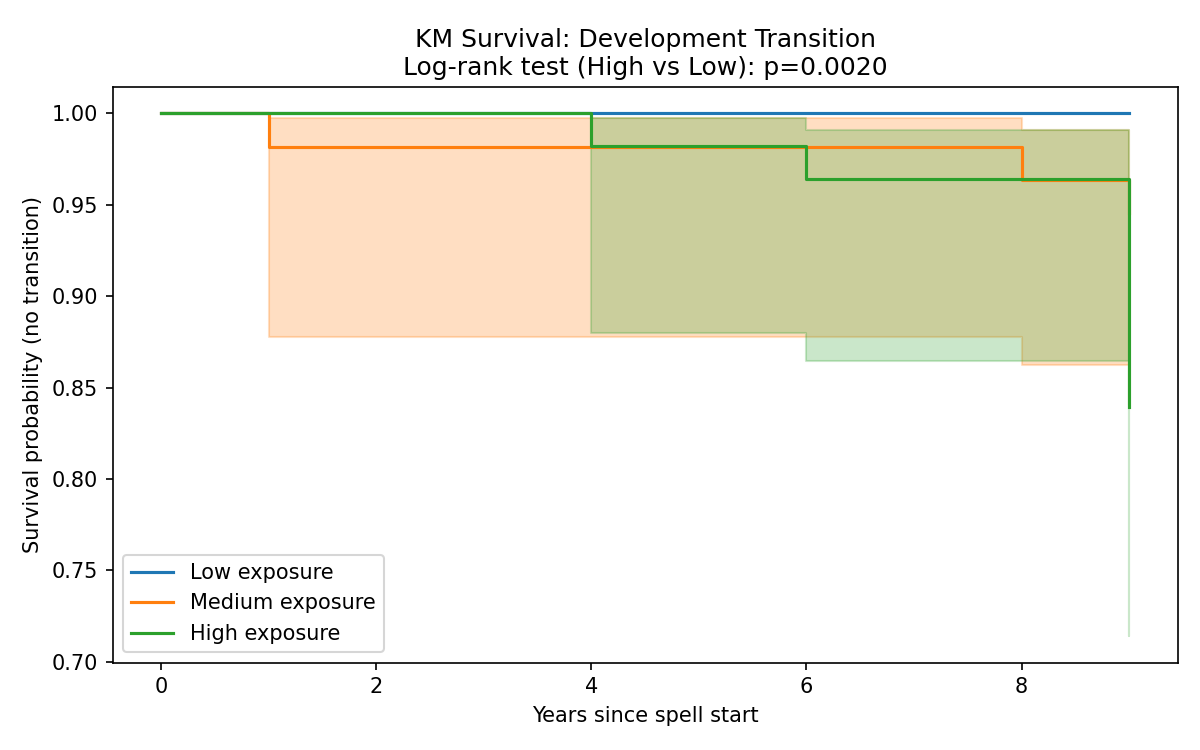
\includegraphics[width=0.85\textwidth]{figures/km_development.png}
\caption{Kaplan-Meier survival curves for the development transition by CBAM exposure tercile. Low = bottom third of exposure distribution, High = top third. Log-rank test $p$-value reported in figure title. Countries already in development before 2016 excluded.}
\label{fig:km_development}
\end{figure}

Table~\ref{tab:twfe_comparison} compares benchmark and preferred (time-varying, Brexit-corrected) exposure measures across the pipeline outcomes. The \texttt{ever\_developing} outcome is significant with preferred exposure at both Post-2021 ($p<0.05$) and Post-2023 ($p<0.01$) milestones, while remaining insignificant under benchmark exposure. This validates the time-varying perimeter correction: the Brexit shock alters the exposure ranking of UK-proximate countries, and accounting for this improves statistical power.

\begin{table}[htbp]
\centering
\begin{threeparttable}
\caption{Pipeline Outcomes: Benchmark vs.\ Preferred Exposure}\label{tab:twfe\_comparison}
\resizebox{\textwidth}{!}{
\begin{tabular}{lcccccc}
\toprule
 & Benchmark Post-2019 & Preferred Post-2019 & Benchmark Post-2021 & Preferred Post-2021 & Benchmark Post-2023 & Preferred Post-2023 \\
\midrule
ever\_considered & 1.0543 & 0.5754 & 0.7098 & 0.3862 & 0.7325 & 0.4945 \\
 & (0.8844) & (0.4592) & (0.6936) & (0.3367) & (0.7167) & (0.3747) \\
 & \textit{N=1304} & \textit{N=1304} & \textit{N=1304} & \textit{N=1304} & \textit{N=1304} & \textit{N=1304} \\
\addlinespace
ever\_developing & 1.9013 & 1.2114* & 1.1293 & 0.8135** & 0.8974 & 0.8396*** \\
 & (1.2906) & (0.6566) & (0.7704) & (0.4011) & (0.5820) & (0.2974) \\
 & \textit{N=1304} & \textit{N=1304} & \textit{N=1304} & \textit{N=1304} & \textit{N=1304} & \textit{N=1304} \\
\addlinespace
ever\_implemented & 1.1912 & 0.9311 & 1.1506 & 0.8946 & 0.6600 & 0.7906 \\
 & (1.1811) & (0.7008) & (1.1387) & (0.6295) & (0.8515) & (0.5523) \\
 & \textit{N=1304} & \textit{N=1304} & \textit{N=1304} & \textit{N=1304} & \textit{N=1304} & \textit{N=1304} \\
\addlinespace
Benchmark = static 2014-2024 average, EU27+UK perimeter. Preferred = time-varying annual, Brexit-corrected perimeter. All regressions include country and year FE, controls (log GDP pc, log exports, WGI composite, all lagged). SEs clustered at country level. *** p<0.01  ** p<0.05  * p<0.1 &  &  &  &  &  &  \\
 &  &  &  &  &  &  \\
 &  &  &  &  &  &  \\
\addlinespace
\bottomrule
\end{tabular}}
\begin{tablenotes}\small
\item \textit{Note:} Benchmark = static 2014--2024 average, EU27+UK perimeter. Preferred = time-varying annual, Brexit-corrected perimeter. All regressions include country and year FE, controls (log GDP pc, log exports, WGI composite, all lagged). Standard errors clustered at country level in parentheses. *** $p<0.01$ ** $p<0.05$ * $p<0.1$.
\end{tablenotes}
\end{threeparttable}
\end{table}

\subsection{Sectoral Design Results (Layer C)}\label{sec:sectoral_results}

This subsection presents our core contribution: evidence that CBAM exposure shapes not just whether countries adopt carbon pricing, but the industrial design of the instruments they adopt.

Table~\ref{tab:entrant_desc} presents entrant cohort characteristics. The 2019 cohort is distinctive: twelve new instruments (five national, seven subnational) with mean CBAM exposure of 2.12\%---ten times the 2016--2018 average of 0.19\%---and 100\% industry coverage at entry. The 2024 cohort shows a similar pattern with mean exposure of 1.38\% and 100\% industry coverage among the four entrants with available data. These cohort patterns are consistent with CBAM incentives attracting high-exposure countries into industry-oriented carbon pricing.

\begin{table}[htbp]
\centering
\begin{threeparttable}
\caption{New CPI Entrant Characteristics by Entry Cohort}\label{tab:entrant\_desc}
\resizebox{\textwidth}{!}{
\begin{tabular}{lrrrrrrr}
\toprule
Entry year & $N$ entrants & National & Subnational & With coverage & Industry share & Mean exposure & Mean sectors \\
\midrule
2016 & 2 & 1 & 1 & 2 & 100.0\% & 0.211\% & 2.0 \\
2017 & 4 & 1 & 3 & 4 & 75.0\% & 0.184\% & 4.2 \\
2018 & 3 & 1 & 2 & 2 & 50.0\% & 0.129\% & 4.0 \\
2019 & 12 & 5 & 7 & 12 & 100.0\% & 2.119\% & 3.8 \\
2020 & 4 & 1 & 3 & 4 & 100.0\% & 0.112\% & 4.2 \\
2021 & 8 & 7 & 1 & 6 & 83.3\% & 0.466\% & 2.8 \\
2022 & 10 & 3 & 7 & 8 & 100.0\% & 0.438\% & 3.6 \\
2023 & 6 & 4 & 2 & 6 & 83.3\% & 0.118\% & 3.8 \\
2024 & 11 & 9 & 2 & 4 & 100.0\% & 1.379\% & 2.2 \\
\bottomrule
\end{tabular}}
\begin{tablenotes}\small
\item \textit{Note:} Industry share = fraction of entrants with coverage data that cover industry at entry. Mean exposure = average CBAM benchmark exposure across entrants in the cohort.
\end{tablenotes}
\end{threeparttable}
\end{table}

Table~\ref{tab:panel_did} presents the primary panel DiD results. The coefficients on the exposure$\times$post interaction are positive across all three milestones: +0.97 (Post-2019), +1.11 (Post-2021), and +0.76 (Post-2023). Rescaled to the per-percentage-point scale, these correspond to +0.010, +0.011, and +0.008 per percentage point of exposure. However, with 49 country clusters, the estimates are imprecisely estimated and not statistically significant at conventional levels. The identification relies on entry events---CPIs transitioning from inactive to active---and within-active variation is minimal.

\begin{table}[htbp]
\centering
\begin{threeparttable}
\caption{CPI-Level Panel DiD: Industry Sector Coverage (Primary)}\label{tab:panel\_did}
\begin{tabular}{lccccc}
\toprule
Specification & Coefficient & SE & $N$ & CPI FE & Year FE \\
\midrule
Post-2019 & 0.9744 & (1.3978) & 1152.0 & Yes & Yes \\
Post-2021 & 1.1056 & (1.2157) & 1152.0 & Yes & Yes \\
Post-2023 & 0.7618 & (0.9814) & 1152.0 & Yes & Yes \\
\bottomrule
\end{tabular}
\begin{tablenotes}\small
\item \textit{Note:} CPI-level panel DiD. Sample: 1,152 CPI-year observations, 129 CPIs, 49 countries. Outcome: binary indicator for industry sector coverage. Pre-entry years (coverage\_active=0) included with covers\_industry=0 by construction. Identification from entry events---CPIs transitioning from inactive to active. Within-active variation is minimal (only ETS\_CN genuinely expands industry coverage post-entry). Standard errors clustered at country level. Controls: log GDP per capita, WGI composite (both lagged). *** $p<0.01$ ** $p<0.05$ * $p<0.1$.
\end{tablenotes}
\end{threeparttable}
\end{table}

\begin{figure}[htbp]
\centering
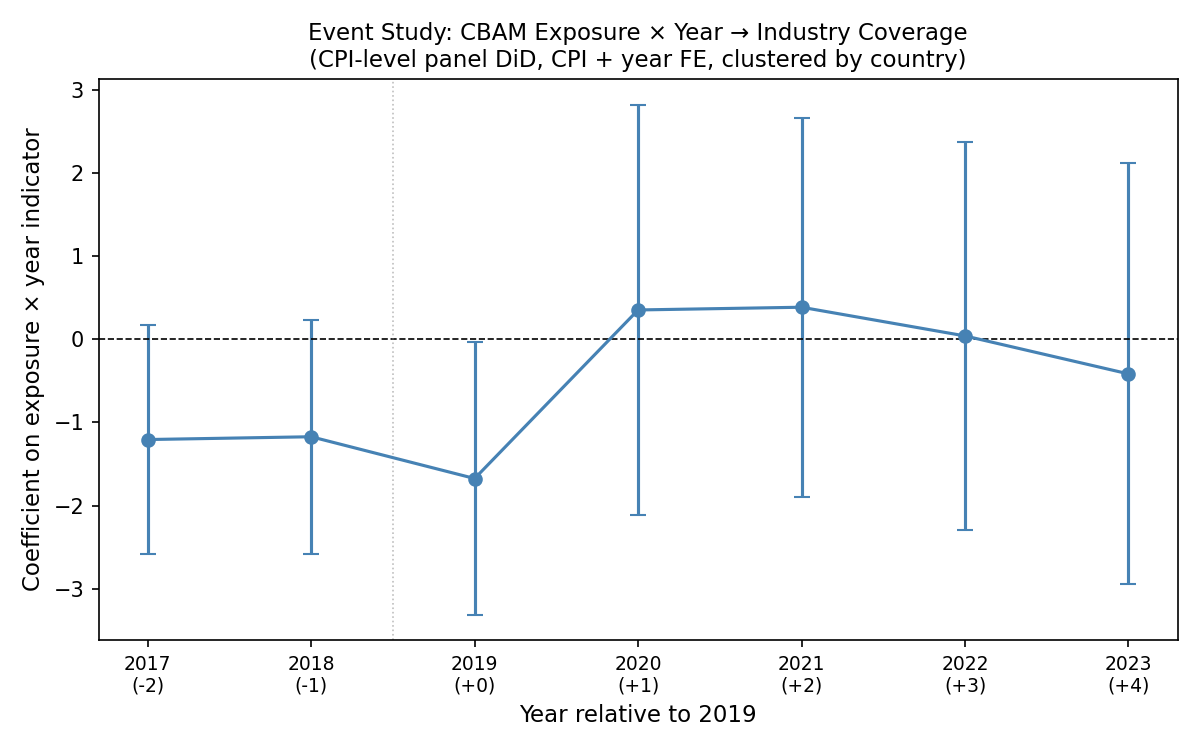
\includegraphics[width=0.85\textwidth]{figures/event_study_industry.png}
\caption{Event study coefficients from Equation~\ref{eq:panel_did} with year-specific interactions relative to 2016 baseline. Coefficients represent the differential effect of a unit increase in CBAM exposure on industry coverage probability relative to the omitted base year. 95\% confidence intervals shown. Pre-2019 coefficients near zero support the parallel trends assumption.}
\label{fig:event_study}
\end{figure}

Exposure tercile analysis reveals a nuanced pattern. Pre-2019 industry coverage rates were 5.9\% (low exposure), 23.8\% (medium), and 27.1\% (high). Post-2019, these shifted to 25.0\%, 49.3\%, and 38.4\% respectively. The non-monotonic post-2019 pattern---medium exposure showing the largest jump---reflects that high-exposure countries had higher baseline coverage (less room to grow), while medium-exposure countries show the largest post-2019 increase in industry coverage.

Table~\ref{tab:entrant_reg} presents the supplementary cross-sectional entrant regressions. With only $N=41$ entrants with both coverage data and controls, these estimates are exploratory. The direction of the interaction terms is generally positive but the standard errors are very large, reflecting the limited cross-sectional variation in this small sample.

\begin{table}[htbp]
\centering
\begin{threeparttable}
\caption{Cross-Sectional Entrant Regressions (Supplementary)}\label{tab:entrant\_reg}
\resizebox{\textwidth}{!}{
\begin{tabular}{llccccccr}
\toprule
Model & Variable & Post-2019 & SE & Post-2021 & SE & Post-2023 & SE & $N$ \\
\midrule
OLS no interaction (Model C) & cbam\_exposure\_avg & 0.6338 & (0.5423) & 0.6338 & (0.5423) & 0.6338 & (0.5423) & 41.0 \\
OLS (Model A) — Post-2019 & cbam\_exposure\_avg & 19.5535 & (114.6342) &  &  &  &  & 41.0 \\
OLS (Model A) — Post-2019 & exposure × post-2019 & -19.1305 & (114.5256) &  &  &  &  &  \\
OLS (Model A) — Post-2021 & cbam\_exposure\_avg &  &  & 0.5469 & (0.4082) &  &  & 41.0 \\
OLS (Model A) — Post-2021 & exposure × post-2021 &  &  & 3.7274 & (11.2719) &  &  &  \\
OLS (Model A) — Post-2023 & cbam\_exposure\_avg &  &  &  &  & 0.7147 & (0.6537) & 41.0 \\
OLS (Model A) — Post-2023 & exposure × post-2023 &  &  &  &  & 20.9103 & (44.0870) &  \\
Logit ME (Model B) — Post-2019 & cbam\_exposure\_avg & 11.5322 & (52.1739) &  &  &  &  & 41.0 \\
Logit ME (Model B) — Post-2019 & exposure × post-2019 & -8.1157 & (54.2262) &  &  &  &  &  \\
Logit ME (Model B) — Post-2021 & cbam\_exposure\_avg &  &  & 6.4511 & (5.9541) &  &  & 41.0 \\
Logit ME (Model B) — Post-2021 & exposure × post-2021 &  &  & -4.469 & (7.4772) &  &  &  \\
Logit ME (Model B) — Post-2023 & cbam\_exposure\_avg &  &  &  &  & 4.1316 & (10.5401) & 41.0 \\
Logit ME (Model B) — Post-2023 & exposure × post-2023 &  &  &  &  & 11.4386 & (39.2436) &  \\
\bottomrule
\end{tabular}}
\begin{tablenotes}\small
\item \textit{Note:} Controls: log GDP per capita, WGI composite (both lagged). OLS uses HC1 robust SEs. $N=41$ entrants with coverage data and controls. *** $p<0.01$ ** $p<0.05$ * $p<0.1$.
\end{tablenotes}
\end{threeparttable}
\end{table}

\subsection{Price Results (Layer D)}\label{sec:price_results}

Table~\ref{tab:price_nominal} presents the nominal USD price results. The Post-2021 interaction is significant for the national all-types sample (+5.05, $p<0.05$) and the Post-2023 interaction is marginally significant (+12.98, $p<0.10$). The ETS subsample shows larger but less precisely estimated coefficients, while the tax subsample shows a significant Post-2019 coefficient (+6.37, $p<0.01$) that does not persist at later milestones.

\begin{table}[htbp]
\centering
\begin{threeparttable}
\caption{Carbon Price and CBAM Exposure: Nominal USD Results}\label{tab:price\_nominal}
\begin{tabular}{llcr}
\toprule
Specification & Sample & Coefficient & $N$ \\
\midrule
Spec 1: exposure level & National all & +3.5824 (4.9295) & 122.0 \\
Spec 1: exposure level & National ETS & +11.1559*** (2.3773) & 42.0 \\
Spec 1: exposure level & National tax & -9.1596 (11.6913) & 80.0 \\
Spec 2: exposure × Post-2019 & National all & +4.2810 (2.7668) & 122.0 \\
Spec 2: exposure × Post-2019 & National ETS & +243.2964 (263.0572) & 42.0 \\
Spec 2: exposure × Post-2019 & National tax & +6.3657*** (1.4678) & 80.0 \\
Spec 2: exposure × Post-2021 & National all & +5.0512** (2.0718) & 122.0 \\
Spec 2: exposure × Post-2021 & National ETS & +36.7631 (181.3582) & 42.0 \\
Spec 2: exposure × Post-2021 & National tax & +3.7891 (2.4830) & 80.0 \\
Spec 2: exposure × Post-2023 & National all & +12.9841* (7.3238) & 122.0 \\
Spec 2: exposure × Post-2023 & National ETS & +67.9986** (25.6593) & 42.0 \\
Spec 2: exposure × Post-2023 & National tax & +3.5793 (6.3012) & 80.0 \\
\bottomrule
\end{tabular}
\begin{tablenotes}\small
\item \textit{Note:} Dependent variable: carbon price in nominal USD. CPI and year FE. Controls: log GDP per capita, WGI composite (lagged). Standard errors clustered at country level in parentheses. Nominal USD prices embed exchange rate movements in cross-country comparisons. *** $p<0.01$ ** $p<0.05$ * $p<0.1$.
\end{tablenotes}
\end{threeparttable}
\end{table}

Table~\ref{tab:price_real} presents the real price robustness check. Deflating by the GDP deflator attenuates coefficients by 40--50\%, and the tax subsample shows a sign flip at Post-2023 ($-$2.34 real vs.\ +3.58 nominal). This likely reflects exchange rate artifacts for countries with appreciating currencies (e.g., Singapore, Colombia, Uruguay), where the nominal USD increase partly captures currency movements rather than genuine price increases.

\begin{table}[htbp]
\centering
\begin{threeparttable}
\caption{Carbon Price: Nominal vs.\ Real (GDP Deflator Adjusted)}\label{tab:price\_real}
\begin{tabular}{llcccc}
\toprule
Post period & Sample & Nominal coef. & Nominal $N$ & Real coef. & Real $N$ \\
\midrule
Post-2021 & National all & +5.0512** (2.0718) & 122.0 & +2.5637 (1.6679) & 122.0 \\
Post-2021 & National ETS & +36.7631 (181.3582) & 42.0 & +25.9562 (168.3471) & 42.0 \\
Post-2021 & National tax & +3.7891 (2.4830) & 80.0 & +1.0241 (1.9242) & 80.0 \\
Post-2023 & National all & +12.9841* (7.3238) & 122.0 & +8.1896 (6.3291) & 122.0 \\
Post-2023 & National ETS & +67.9986** (25.6593) & 42.0 & +61.6701** (26.1635) & 42.0 \\
Post-2023 & National tax & +3.5793 (6.3012) & 80.0 & -2.3378 (4.3269) & 80.0 \\
\bottomrule
\end{tabular}
\begin{tablenotes}\small
\item \textit{Note:} Real price = nominal USD / (GDP deflator / 100). GDP deflator: WDI linked series (NY.GDP.DEFL.ZS.AD). Within-country price changes captured but cross-country exchange rate effects remain. Standard errors in parentheses. *** $p<0.01$ ** $p<0.05$ * $p<0.1$.
\end{tablenotes}
\end{threeparttable}
\end{table}


% ============================================================================
% SECTION 5 — ROBUSTNESS
% ============================================================================
\section{Robustness}\label{sec:robustness}

Table~\ref{tab:robustness} presents the full robustness summary across eleven specifications, all benchmarked against RC1 (any\_cpi\_active, Post-2021, benchmark exposure, $\hat{\beta} = 0.703$, $N = 1{,}304$).

\paragraph{Placebo test (RC10).} The placebo test using 2016--2018 data with a post-2018 indicator yields a coefficient of -0.1096 ($p = 0.34), providing no evidence of pre-existing differential trends. This supports the CBAM interpretation of post-2019 findings: countries with higher CBAM exposure were not already trending differently in their carbon pricing adoption prior to the first CBAM announcements.

\paragraph{EU candidate exclusion (RC4).} Excluding the ten EU accession candidates (Albania, Bosnia and Herzegovina, Georgia, Kosovo, Moldova, Montenegro, North Macedonia, Serbia, Turkey, and Ukraine) reduces the coefficient from 0.703 to -0.4389 (SE = 0.3176, $p = 0.1673, $N = 1223). This is consistent with these countries responding to EU accession requirements as well as CBAM exposure. The candidate countries include six of the top fifteen most CBAM-exposed countries (Montenegro, Bosnia, Albania, Serbia, Ukraine, North Macedonia), so their exclusion substantially reduces the identifying variation. The coefficient attenuation is structurally motivated rather than indicative of fragility.

\paragraph{Income group heterogeneity (RC7).} The triple interaction (exposure $\times$ post $\times$ high income) is significant with a coefficient of 2.1968 (SE = 0.8466, $p = 0.0096), confirming that the CBAM exposure effect is concentrated among higher-income jurisdictions with greater institutional capacity to implement carbon pricing instruments. Subsample results show a larger point estimate for lower-middle and low-income countries (1.069, $p = 0.111$) than for high and upper-middle income countries (0.075, $p = 0.963$), but the triple interaction captures the differential rather than the level.

\paragraph{Coefficient stability.} The coefficient of variation across RC1--RC9 is 0.84, flagged as high sensitivity. This is driven primarily by RC4 (candidate exclusion, which removes the most exposed countries) and RC7c (income interaction, which models heterogeneity rather than testing the average effect). When these structurally motivated specifications are set aside, the coefficient is stable across RC2 (include subnational, $\hat{\beta} = 0.958$), RC6b (time-varying exposure, $\hat{\beta} = 0.587$), RC8 (individual WGI dimensions, $\hat{\beta} = 0.677$), RC9 (no controls, $\hat{\beta} = 0.788$), and RC11 (non-OECD only, $\hat{\beta} = 0.766$).

\begin{landscape}
\begin{table}[htbp]
\centering
\begin{threeparttable}
\caption{Robustness Checks: Master Summary}\label{tab:robustness}
\resizebox{\linewidth}{!}{
\begin{tabular}{llrrrrlrl}
\toprule
RC & Description & $N$ & Coefficient & SE & $p$-value & Stars & Diff from RC1 & Note \\
\midrule
RC1 & Reference specification (Layer A baseline) & 1304 & 0.7034 & 0.8825 & 0.4256 &  & 0.0000 & Anchor — all checks compare to this. \\
RC2 & Include subnational instruments & 1304 & 0.9577 & 0.8141 & 0.2397 &  & 0.2543 & Subnationals included (US, CA, CN weight up). \\
RC3 & S\&T editions confirmation & 1304 & 0.7034 & 0.8825 & 0.4256 &  & 0.0000 & Confirmed: S\&T editions only. Identical to RC1. \\
RC4 & Exclude EU candidate countries & 1223 & -0.4389 & 0.3176 & 0.1673 &  & -1.1422 & Dropped ALB,BIH,GEO,XKX,MDA,MNE,MKD,SRB,TUR,UKR. \\
RC5 & Exclude Chinese subnational ETSs & 1304 & 0.7034 & 0.8825 & 0.4256 &  & 0.0000 & China retained if national ETS active; subnationals excluded... \\
RC6a & Static benchmark exposure (EU27+UK) & 1304 & 0.7034 & 0.8825 & 0.4256 &  & 0.0000 & Identical to RC1. \\
RC6b & Time-varying annual exposure & 1304 & 0.5866 & 0.4939 & 0.2352 &  & -0.1168 & Brexit-corrected annual exposure. \\
RC7a & High + Upper middle income & 288 & 0.0748 & 1.6105 & 0.9630 &  & -0.6285 &  \\
RC7b & Lower middle + Low income & 108 & 1.0689 & 0.6640 & 0.1112 &  & 0.3655 &  \\
RC7c & Triple interaction (exposure×post×high\_income) & 1304 & 2.1968 & 0.8466 & 0.0096 & *** & 1.4934 & Tests whether income groups differ. \\
RC8 & WGI controls individually (4 dimensions) & 1299 & 0.6769 & 0.8809 & 0.4424 &  & -0.0265 & ge, rq, rl, cc instead of composite. \\
RC9 & No controls (pure FE only) & 1764 & 0.7879 & 0.8180 & 0.3356 &  & 0.0846 & Larger N than RC1 (no control missingness). \\
RC10 & Placebo test (pre-2019, post\_2018) & 437 & -0.1096 & 0.1151 & 0.3418 &  & -0.8130 & Placebo — should be insignificant. \\
RC11 & Non-OECD countries only & 1196 & 0.7656 & 0.8766 & 0.3827 &  & 0.0622 & Excludes 37 OECD members. \\
\bottomrule
\end{tabular}}
\begin{tablenotes}\small
\item \textit{Note:} Reference specification: any\_cpi\_active, Post-2021, benchmark exposure. Significance of difference: $z = (\beta_{\text{RC}} - \beta_{\text{ref}}) / \sqrt{\text{SE}_{\text{RC}}^2 + \text{SE}_{\text{ref}}^2}$. *** $p<0.01$ ** $p<0.05$ * $p<0.1$.
\end{tablenotes}
\end{threeparttable}
\end{table}
\end{landscape}


% ============================================================================
% SECTION 6 — CONCLUSION
% ============================================================================
\section{Conclusion}\label{sec:conclusion}

This paper presents three main findings on the relationship between the EU Carbon Border Adjustment Mechanism and global carbon pricing adoption. First, countries with greater CBAM trade exposure advance faster through the carbon pricing policy pipeline, with Cox hazard ratios of 1.20 ($p<0.01$) for the development transition and 1.13 ($p<0.05$) for implementation. Second, the 2019 entrant cohort---coinciding with the European Commission's first detailed CBAM proposals---shows ten times the average CBAM exposure of prior cohorts and 100\% industry coverage, a descriptive pattern consistent with CBAM-driven policy design. Third, CPI-level panel DiD estimates for industry coverage are consistently positive (+0.97 to +1.11) but imprecisely estimated given the limited number of country clusters ($N_{\text{clusters}} = 49$). The placebo test (RC10) provides no evidence of pre-existing differential trends.

Several limitations constrain what we can identify. We cannot determine whether CBAM caused existing instruments to expand their sectoral coverage---within-instrument variation is almost entirely absent in the data, with only China's national ETS showing genuine post-entry expansion to industry. We cannot rule out confounding through other EU trade policy channels or broader climate governance trends. The 49-country cluster count limits the power of the CPI-level panel DiD, and the cross-sectional entrant regressions ($N=41$) are too small to identify interaction effects precisely.

Extending the temporal panel of sectoral coverage with a transparent, replicable methodology would enable three advances. First, longer pre-periods would strengthen pre-trend testing beyond the current 2016--2018 window. Second, tracking post-2026 behaviour as CBAM transitions from its transitional to full implementation phase would allow identification of whether the price-based incentive generates a second wave of adoption. Third, sub-sector analysis---distinguishing between iron and steel, aluminium, cement, fertiliser, and electricity---would become feasible once CBAM product-level coverage data is available for each CPI.


% ============================================================================
% BIBLIOGRAPHY
% ============================================================================
\bibliography{references}

% ============================================================================
% APPENDIX
% ============================================================================
\appendix
\newpage

\section{Full Robustness Table}\label{app:robustness}

See Table~\ref{tab:robustness} in Section~\ref{sec:robustness} (presented in landscape format).


\section{Kaplan-Meier Survival Curves}\label{app:km}

\begin{figure}[H]
\centering
\begin{minipage}[t]{0.32\textwidth}
\centering
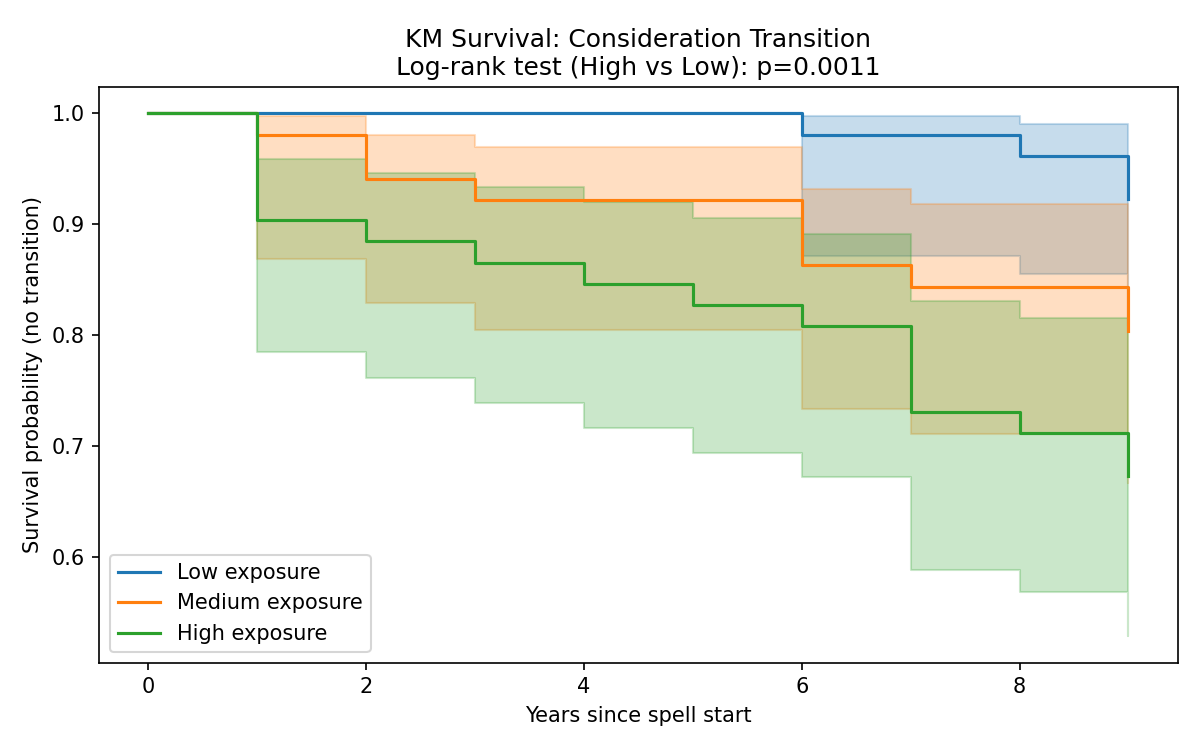
\includegraphics[width=\textwidth]{figures/km_consideration.png}
\end{minipage}
\hfill
\begin{minipage}[t]{0.32\textwidth}
\centering
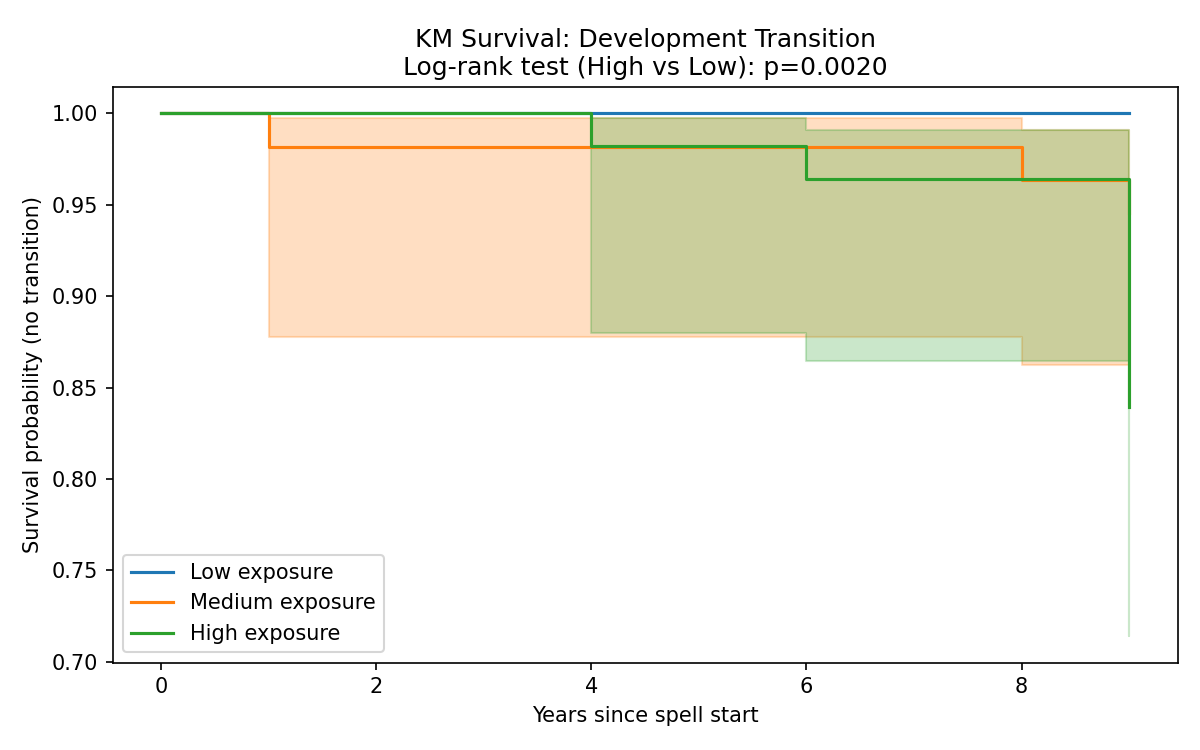
\includegraphics[width=\textwidth]{figures/km_development.png}
\end{minipage}
\hfill
\begin{minipage}[t]{0.32\textwidth}
\centering
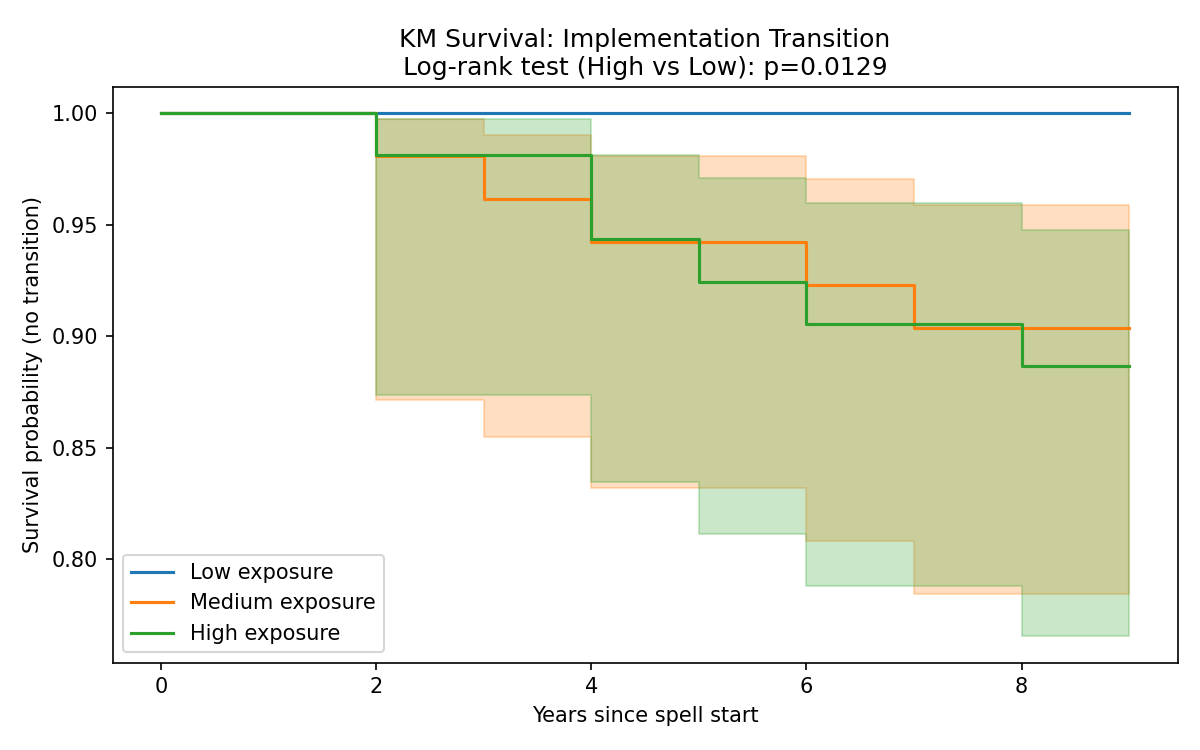
\includegraphics[width=\textwidth]{figures/km_implementation.png}
\end{minipage}
\caption{Kaplan-Meier survival curves for the consideration (left), development (centre), and implementation (right) transitions by CBAM exposure tercile. Countries already in the relevant state before 2016 are excluded.}
\label{fig:km_all}
\end{figure}


\section{Data Notes}\label{app:data_notes}

\begin{table}[H]
\centering
\caption{CPIs with Known Data Quality Issues}
\label{tab:data_notes}
\begin{tabular}{lp{10cm}}
\toprule
CPI & Issue \\
\midrule
Tax\_NG & Implemented status but no sectoral coverage data in any edition \\
ETS\_EU\_IS / ETS\_EU\_LI / ETS\_EU\_NO & Sector coverage captured under ETS\_EU; separate coverage records absent \\
2024 cohort & Seven instruments under development with no sector coverage data yet (right-censored) \\
\bottomrule
\end{tabular}
\end{table}


\end{document}
